\documentclass[11pt, oneside]{article}   	% use "amsart" instead of "article" for AMSLaTeX format
\usepackage{geometry}                		% See geometry.pdf to learn the layout options. There are lots.
\geometry{letterpaper}                   		% ... or a4paper or a5paper or ... 
%\geometry{landscape}                		% Activate for rotated page geometry
%\usepackage[parfill]{parskip}    		% Activate to begin paragraphs with an empty line rather than an indent
\usepackage{graphicx}				% Use pdf, png, jpg, or eps§ with pdflatex; use eps in DVI mode
\graphicspath{ {/home/user/shujialiang/documents/research\ limmer\ lab/} }			% TeX will automatically convert eps --> pdf in pdflatex		
\usepackage{amssymb}

%SetFonts

%SetFonts


\title{Problem Set 8 Solution}
\author{Shujia Liang}
%\date{}							% Activate to display a given date or no date

\begin{document}
\maketitle
\section{Problem 1}
\subsection{}
We consider $J(q, t)$ as a function describing the instant fraction of particles passing point q at a given time. Specifically, $J({q_B}, t)$ describes the leaving probability density at $q_B$, as we regard $q_B$ as an absorption state. Thus $\phi_B$ is the total probability left from $q_B$ across time, which is the splitting probability. $p(q, 0)$ shows the initial case where the starting point is $q_0$ or not, yet $p(q_A, t)$ and $p(q_B, t)$ only show that both $q_A$ and $q_B$ are absorbing states. 

\subsection{}
$$\int_{0}^{\infty} dt \frac{dp}{dt} = -\int_{0}^{\infty} dt \frac{\partial {J(q, t)}}{\partial t}$$
$$p(q, \infty)-p(q, 0) = -\int_{0}^{\infty} dt \frac{\partial {J(q, t)}}{\partial t}$$
$$p(q, \infty)-\delta (q-q_0) = -\int_{0}^{\infty} dt \frac{\partial {J(q, t)}}{\partial t}$$
$$\delta (q-q_0) = \int_{0}^{\infty} dt \frac{\partial {J(q, t)}}{\partial t}$$
as in infinite amount of time all probability density is extinct due to non-zero probability of edge cases.
\subsection{}
$$\int_{q}^{q_B}\delta (q-q_0) = \int_{0}^{\infty} dt \int_{q}^{q_B} dx \frac{\partial {J(x, t)}}{\partial x}$$
$$\Theta(q_0, q) = \phi_B(q_0)-\int_{0}^{\infty} dt J(q, t)$$
Splitting probability occurs.
\subsection{}
$$\int_{q_A}^{q_B} dq \Theta(q_0, q) = \int_{q_A}^{q_0} dq e^{\beta w(q)}$$
$\int_{0}^{\infty} dt J(q, t)$ is zero when integrated after multiplied by Boltzmann factor, since the Boltzmann factor cancels from the definition of J in (2), and thus the integration of such an odd function becomes zero, and the only thing left is $\phi_B \int_{q_A}^{q_B} dq e^{\beta w(q)}$, and thus $$\phi_B = \int_{q_A}^{q_0} dq e^{\beta w(q)} / \int_{q_A}^{q_B} dq e^{\beta w(q)}$$
\subsection{}
Plug in the error function, we finalize the result to be $$1-\frac{1}{2}erfc(-\sqrt{\frac{1}{2}\beta m}\omega q_0)$$ as erfc($-\infty$) is simply 2.
\subsection{}
In this graph below, we discover the crossover region (between 0.1 and 0.9) to be $[-\frac{1}{\sqrt{\frac{1}{2}m\omega^{2}/k_B T}}, \frac{1}{\sqrt{\frac{1}{2}m\omega^{2}/k_B T}}]$. Such crossover region should be within a $k_B T$ of the peak of barrier.

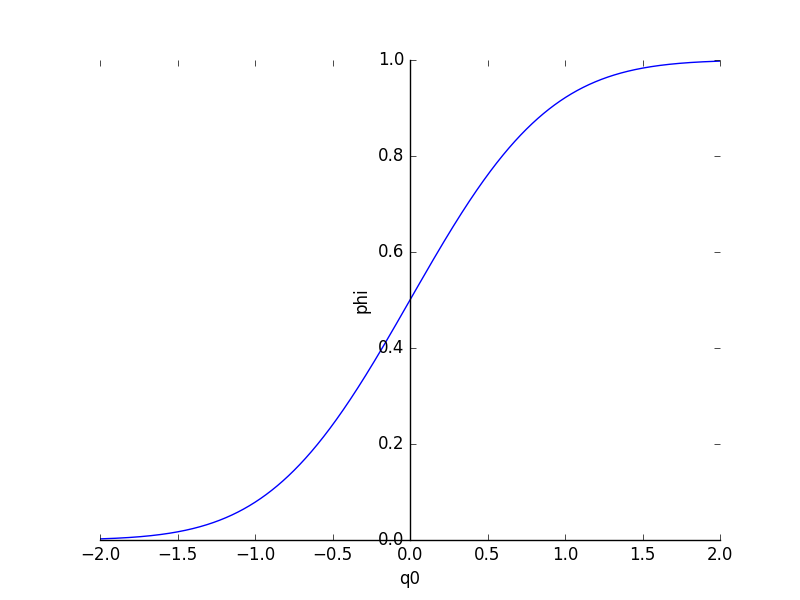
\includegraphics[scale = 0.5]{error function.png}

\section{Problem 2}
\subsection{}
Notice the definition of R, $$\gamma (q(t+\Delta t)-q(t))/\Delta t = -\frac{dw}{dq}+\eta$$
$$ q(t+\Delta t) = q(t) - \frac{1}{\gamma} \frac{dw}{dq} \Delta t + R$$

\subsection{}
$$<R^2> = <\gamma^{-1} \int_{t}^{t+\Delta t} dt' \gamma^{-1} \int_{t}^{t+\Delta t} dt'' \eta (t') \eta (t'')>$$
$$   = \gamma^{-2} \int_{t}^{t+\Delta t} \int_{t}^{t+\Delta t} dt'dt'' <\eta (t') \eta (t'')>$$
$$   = \gamma^{-1} \int_{t}^{t+\Delta t} \int_{t}^{t+\Delta t} dt'dt'' 2k_B T\delta (t'-t'')$$
$$   = 2k_B T\Delta t /\gamma$$
$$   = 2D\Delta t$$

\subsection{}
In this case, from $\gamma \dot{q} = -\frac{dw}{dq} + \eta = \overline{F} + \eta$, we integrate left side to get 
$$ q(t) - q(0) = \eta ^{-1} \overline{F}t + \eta ^{-1} \int_{0}^{t} dt'\eta (t')$$
Since $\beta = \frac{1}{k_B T}$ and $D = \frac{1}{ \beta \gamma}$, $<q(t) - q(0)>/t = \gamma ^{-1} \overline{F} = \beta D\overline{F}$
as the average of $\eta$ is 0 overall.

\subsection{}
Simulation shows 10000 repeats with $\Delta t= 0.001$
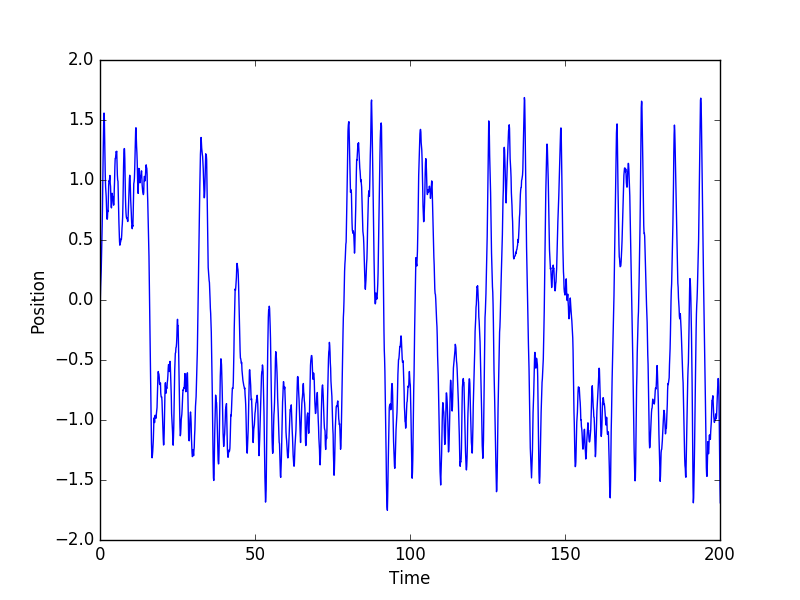
\includegraphics[scale = 0.5]{qvst.png}

\subsection{}
Histogram of q from the data above
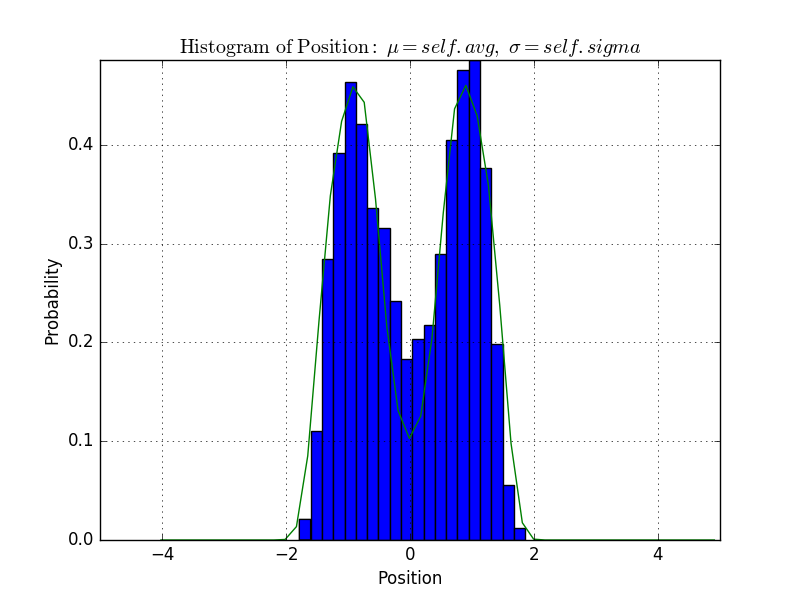
\includegraphics[scale = 0.5]{hist4.png}

\subsection{}
\paragraph{}
$k_B T = 0.2$
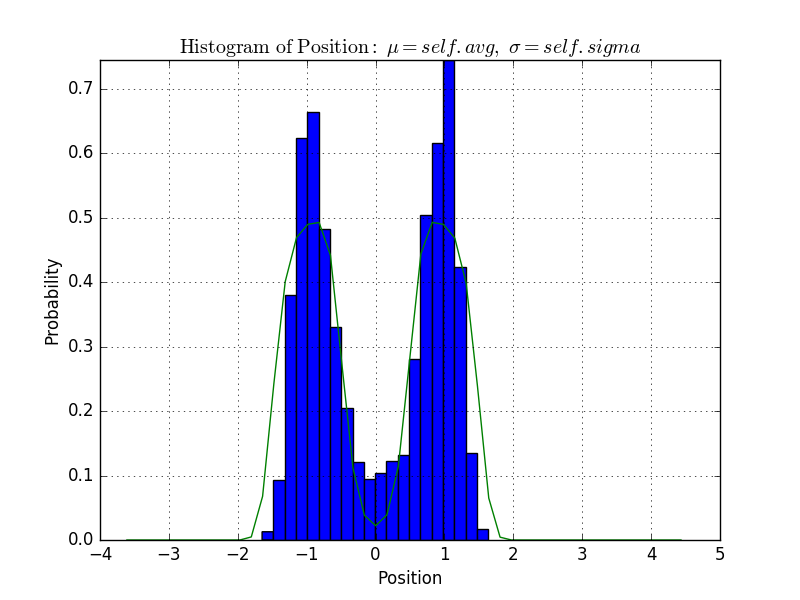
\includegraphics[scale = 0.5]{hist2.png}
\paragraph{}
$k_B T = 0.1$
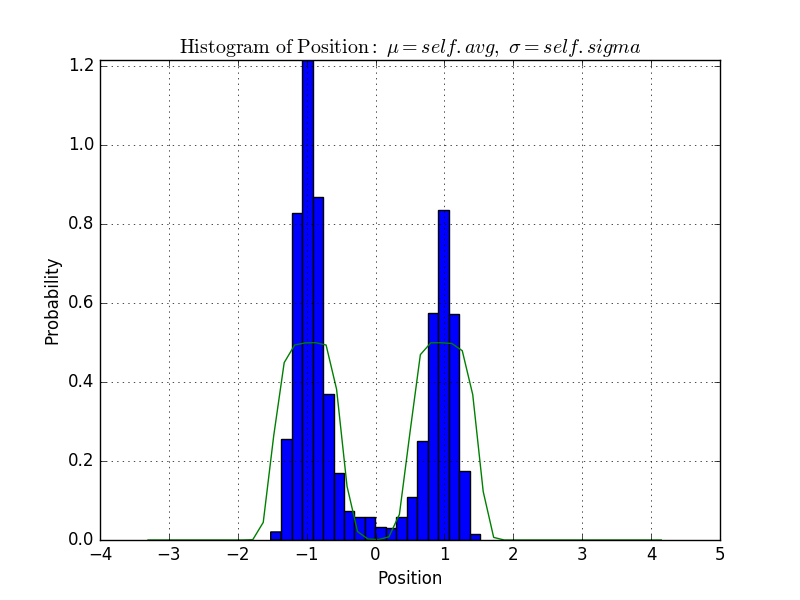
\includegraphics[scale = 0.5]{hist1.png}
\paragraph{}
$k_B T = 0.05$
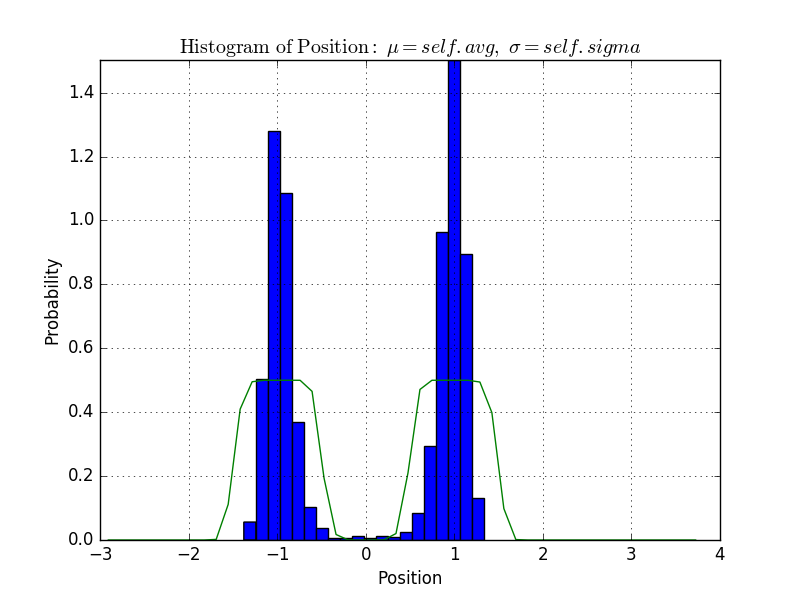
\includegraphics[scale = 0.5]{hist5.png}

The middle barrow increases with smaller $k_B T$ and the peak height becomes sharper. I expect coherency of Boltzmann distribution and Langevin, and the algorithm sounds inaccurate for the Boltzmann distribution. Similar situation applies in next question, which the error should increase with increasing $\Delta t$.

\subsection{}
\paragraph{}
$\Delta t = 0.01$
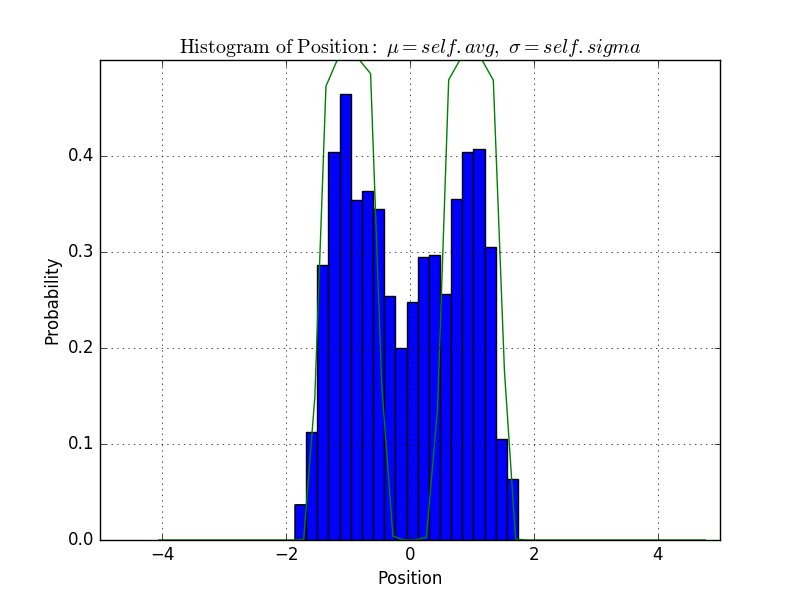
\includegraphics[scale = 0.5]{dt1.png}
\paragraph{}
$\Delta t = 0.02$
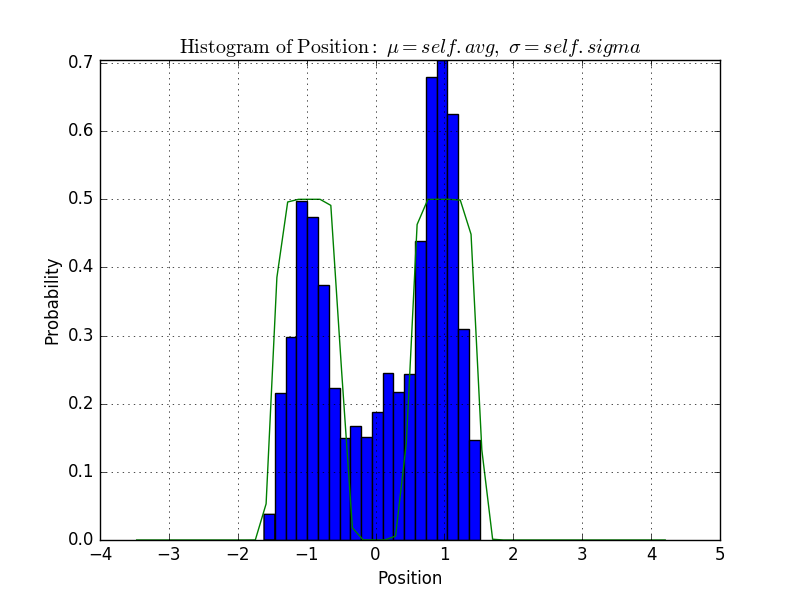
\includegraphics[scale = 0.5]{dt2.png}
\paragraph{}
$\Delta t = 0.03$
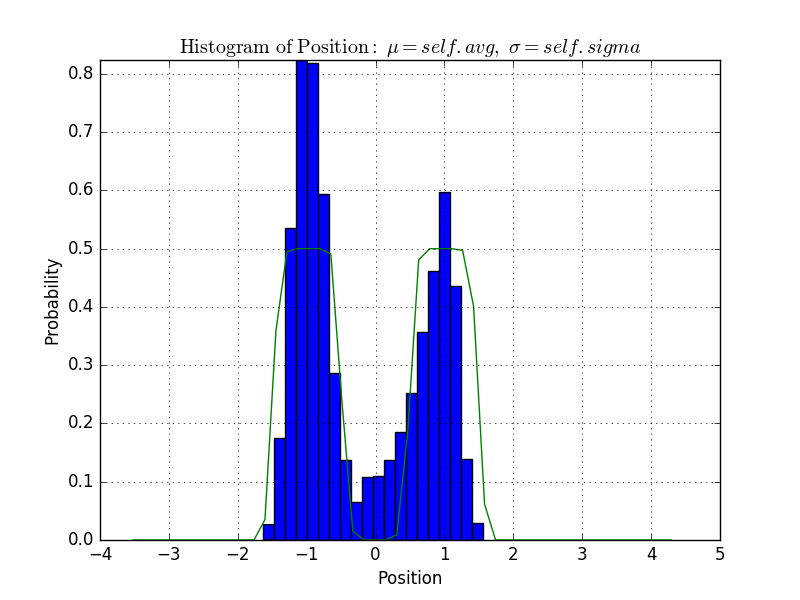
\includegraphics[scale = 0.5]{dt3.png}

\section{Problem 3}
\subsection{}
Splitting probability as a function of $q_0$:
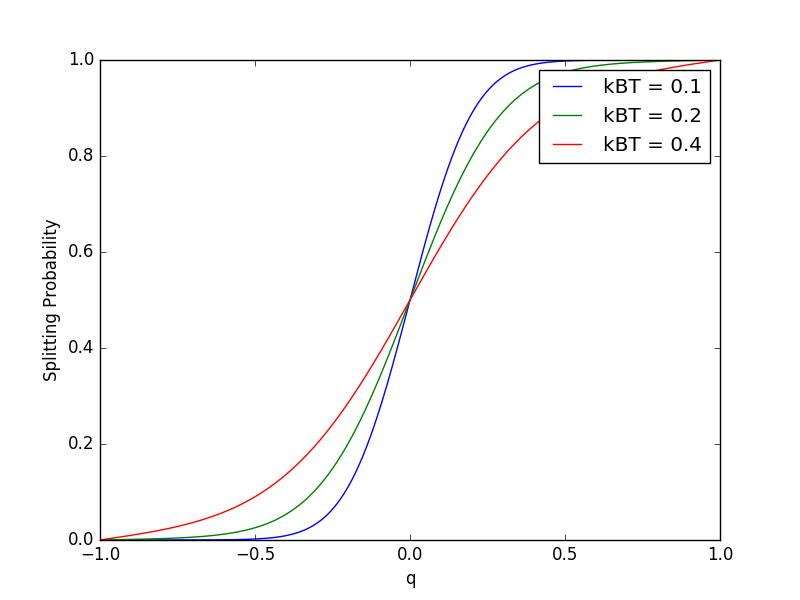
\includegraphics[scale = 0.5]{Onsager.png}

\subsection{}
Comparison between Onsager and Harmonic Oscillator.
\paragraph{}
$k_B T = 0.1$
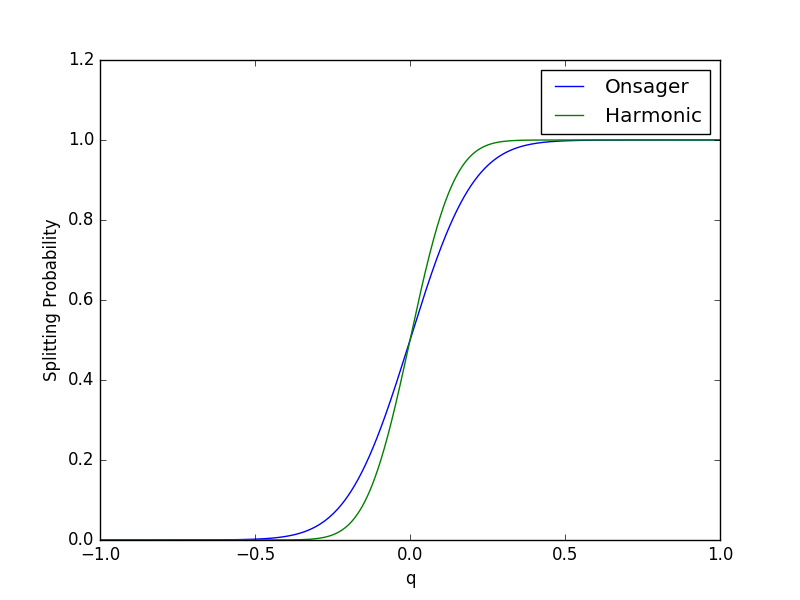
\includegraphics[scale = 0.5]{kbt1.png}

\paragraph{}
$k_B T = 0.2$
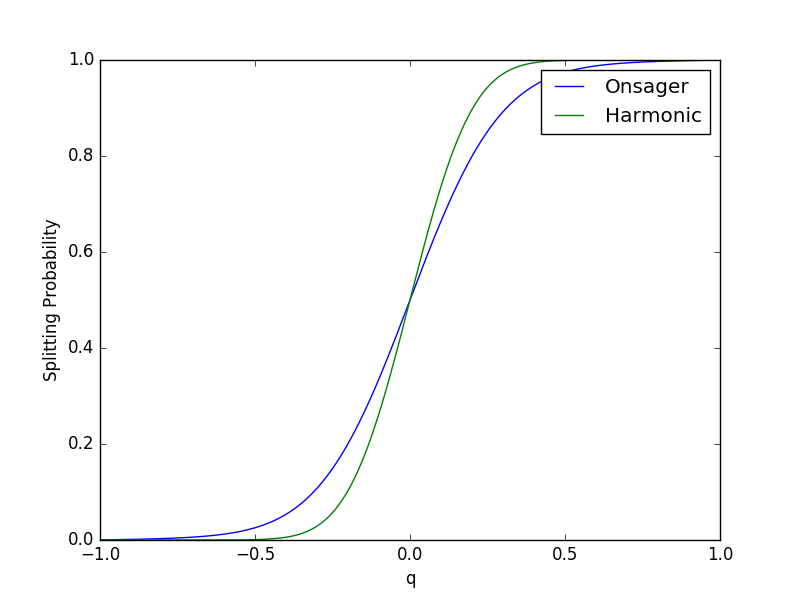
\includegraphics[scale = 0.5]{kbt2.png}

\paragraph{}
$k_B T = 0.4$
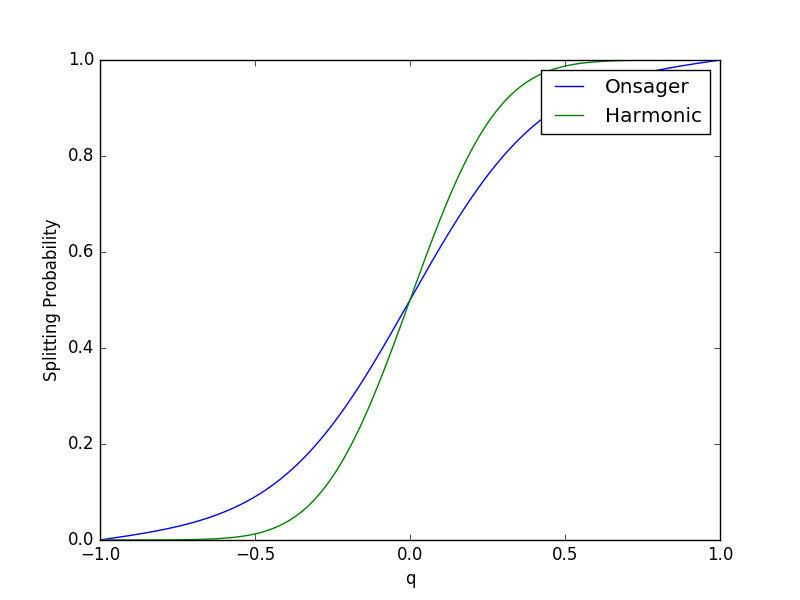
\includegraphics[scale = 0.5]{kbt4.png}

\end{document}  